%!TEX root = project.tex

\chapter*{About this project}
\paragraph{Abstract}
Competitive online gaming has seen a significant increase in popularity in recent times, whether watching or participating, competitive games can consume a large portion of our free time. Organising tournaments require organisation and rules. To ensure the rules are upheld require some form of administration from a system or individual. Issues can occur when an individual is responsible for managing these tournaments, for example, if a tournament has a fixed schedule but the person responsible for managing the tournament is unavailable, then the tournament game must be postponed. Administrators are also required to ensure matchmaking fairness between teams which can be very time consuming and inefficient.

\paragraph{Authors}
Ethan Horrrigan



\chapter{Introduction}
Competitive online gaming has seen a significant increase in popularity in recent times. The estimated global esports audience was estimated at 335 million people in 2017 generating a revenue of more than \$900M with an estimated growth of over \$1600M in 2021.~\cite{sjoblom2019esports} Yuri Seo and Sang-Uk Jung ~\cite{seo2016beyond} outlined why people play or spectate competitive games. The main factors include entertainment and gaining a better understanding of a game. Whether spectating or participating, competitive games can consume a large portion of our free time. Organising tournaments require organisation and rules. To ensure the rules are upheld require some form of administration from a system or an individual. Issues can occur when an individual is responsible for managing these tournaments, for example, if a tournament has a fixed schedule but the person responsible for managing the tournament is unavailable, then the tournament game must be postponed. Administrators are also required to ensure matchmaking fairness between teams which can be very time consuming and inefficient. The disadvantages of physical tournaments do not exist in an online game

\chapter{Context}
\begin{itemize}
	\item Provide a context for your project.
	\item Set out the objectives of the project
	\item Briefly list each chapter / section and provide a 1-2 line description of what each section contains.
	\item List the resource URL (GitHub address) for the project and provide a brief list of the main elements at the URL.
\end{itemize}

\section{League of Legends}
League of Legends is a free-to-play multiplayer online battle arena (MOBA). A match is played between two teams, each consisting of five players and five roles. each player is responsible for picking a role. The main objective of the game is for players to defend their base and attempt to destroy their opponents’.
\begin{center}    
	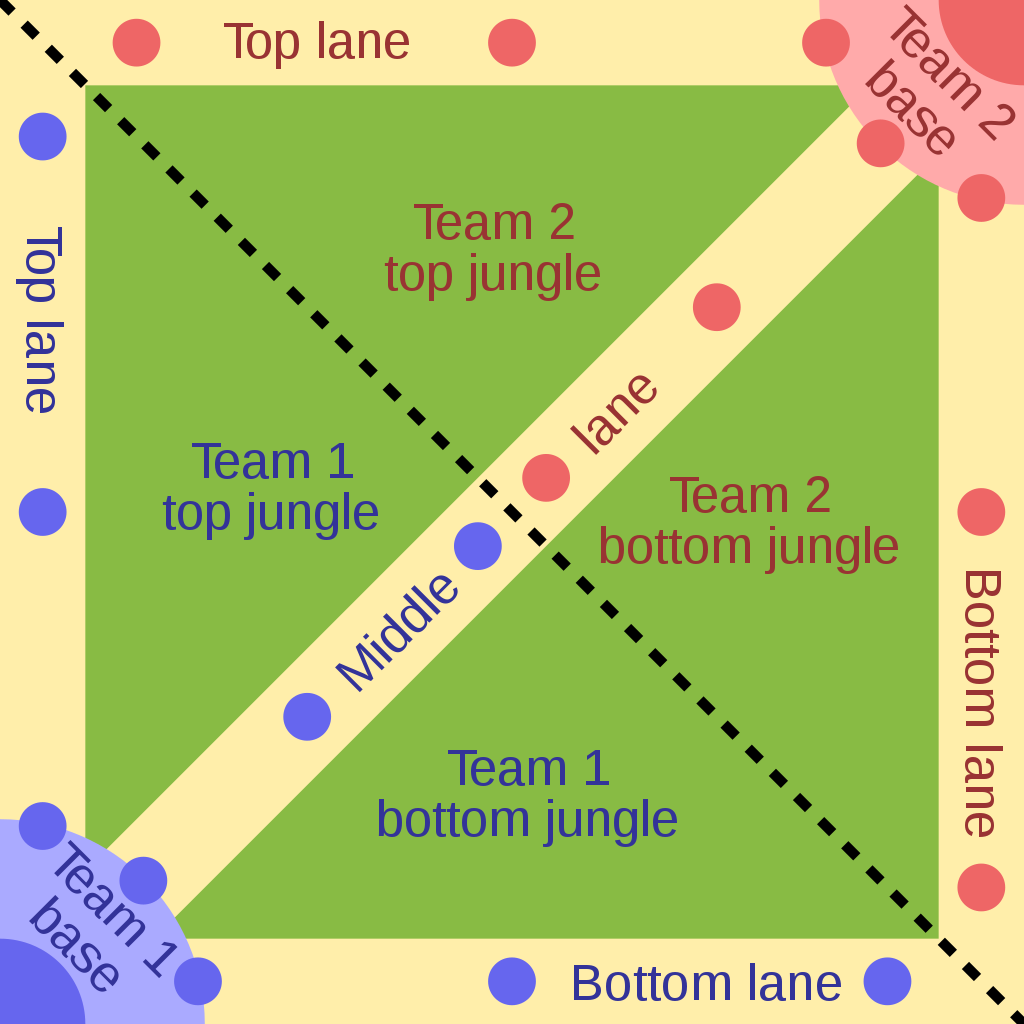
\includegraphics[width=8cm,height=4.3cm,keepaspectratio]{img/Map.png}
\end{center}

Quisque vel erat a justo volutpat auctor a nec odio. Sed rhoncus augue sit amet nisl tincidunt, vitae cursus tellus efficitur. Class aptent taciti sociosqu ad litora torquent per conubia nostra, per inceptos himenaeos. Pellentesque et auctor dui. Fusce ornare odio ipsum, et laoreet mi molestie sed. Cras at massa sit amet ipsum gravida aliquam. Nulla suscipit porta imperdiet. Fusce eros neque, bibendum sit amet consequat non, pulvinar quis ipsum.

\subsection{More filler}
Donec fermentum sapien ac rhoncus egestas. Nullam condimentum condimentum eros sit amet semper. Nam maximus condimentum ligula. Praesent faucibus in nisi vitae tempus. Sed pellentesque eleifend ante, ac malesuada nibh dapibus nec. Phasellus nisi erat, pulvinar vel sagittis sed, auctor et magna. Quisque finibus augue elit, consequat dignissim purus mollis nec. Duis ultricies euismod tortor, nec sodales libero pellentesque et. Interdum et malesuada fames ac ante ipsum primis in faucibus.

Donec id interdum felis, in semper lacus. Mauris volutpat justo at ex dignissim, sit amet viverra massa pellentesque. Suspendisse potenti. Praesent sit amet ipsum non nibh eleifend pretium. In pretium sapien quam, nec pretium leo consequat nec. Pellentesque non dui lacus. Aenean sed massa lacinia, vehicula ante et, sagittis leo. Sed nec nisl ac tellus scelerisque consequat. Ut arcu metus, eleifend rhoncus sapien sed, consequat tincidunt erat. Cras ut vulputate ipsum.

Curabitur et efficitur augue. Proin condimentum ultrices facilisis. Mauris nisi ante, ultrices sed libero eget, ultrices malesuada augue. Morbi libero magna, faucibus in nunc vitae, ultricies efficitur nisl. Donec eleifend elementum massa, sed eleifend velit aliquet gravida. In ac mattis est, quis sodales neque. Etiam finibus quis tortor eu consequat. Nullam condimentum est eget pulvinar ultricies. Suspendisse ut maximus quam, sed rhoncus urna.

\section{Filler}
Phasellus eu tellus tristique nulla porttitor convallis. Vestibulum ac est eget diam mollis consectetur. Donec egestas facilisis consectetur. Donec magna orci, dignissim vel sem quis, efficitur condimentum felis. Donec mollis leo a nulla imperdiet, in bibendum augue varius. Quisque molestie massa enim, vitae ornare lacus imperdiet non. Donec et ipsum id ante imperdiet mollis. Nullam est est, euismod sit amet cursus a, feugiat a lectus. Integer sed mauris dolor.

Mauris blandit neque tortor, consequat aliquam nisi aliquam vitae. Integer urna dolor, fermentum ut iaculis ut, semper eu lacus. Curabitur mollis at lectus at venenatis. Donec fringilla diam ac risus imperdiet suscipit. Aliquam convallis quam vitae turpis interdum, quis pharetra lacus tincidunt. Nam dictum maximus lectus, vitae faucibus ante. Morbi accumsan velit nec massa tincidunt porttitor. Nullam gravida at justo id viverra. Mauris ante nulla, eleifend vitae sem vitae, porttitor lobortis eros.

Cras tincidunt elit id nisi aliquam, id convallis ex bibendum. Sed vel odio fringilla, congue leo quis, aliquam metus. Nunc tempor vehicula lorem eu ultrices. Curabitur at libero luctus, gravida lectus sed, viverra mi. Cras ultrices aliquet elementum. Pellentesque habitant morbi tristique senectus et netus et malesuada fames ac turpis egestas. Sed metus ante, suscipit sit amet finibus ut, gravida et orci. Nunc est odio, luctus quis diam in, porta molestie magna. Interdum et malesuada fames ac ante ipsum primis in faucibus. Mauris pulvinar lacus odio, luctus tincidunt magna auctor ut. Ut fermentum nisl rhoncus, tempus nulla eget, faucibus tortor. Suspendisse eu ex nec nunc mollis pulvinar. Nunc luctus tempus tellus eleifend porta. Nulla scelerisque porttitor turpis porttitor mollis.

Duis elementum efficitur auctor. Nam nisi nulla, fermentum sed arcu vel, posuere semper dui. Fusce ac imperdiet felis. Aenean quis vestibulum nisl. Integer sit amet tristique neque, at suscipit tortor. Morbi et placerat ante, vel molestie dui. Vivamus in nibh eget massa facilisis accumsan. Nunc et purus ac urna fermentum ultrices eget sit amet justo. Class aptent taciti sociosqu ad litora torquent per conubia nostra, per inceptos himenaeos. Cras elementum dui nunc, ac tempor odio semper et. Ut est ipsum, sollicitudin eleifend nisl eu, scelerisque cursus nunc. Nam at lectus vulputate, volutpat tellus vel, pharetra mauris. Integer at aliquam massa, at iaculis sem. Morbi nec imperdiet odio. In hac habitasse platea dictumst.

Mauris a neque lobortis, venenatis erat ut, eleifend quam. Nullam tincidunt tellus quis ligula bibendum, a malesuada erat gravida. Phasellus eget tellus non risus tincidunt sagittis condimentum quis enim. Donec feugiat sapien sit amet tincidunt fringilla. Vivamus in urna accumsan, vehicula sem in, sodales mauris. Aenean odio eros, tristique non varius id, tincidunt et neque. Maecenas tempor, ipsum et sollicitudin rhoncus, nibh eros tempus dolor, vitae dictum justo massa in eros. Proin nec lorem urna. In ullamcorper vitae felis sit amet tincidunt. Maecenas consectetur iaculis est, eu finibus mi scelerisque et. Nulla id ex varius, ultrices eros nec, luctus est. Aenean ac ex eget dui pretium mattis. Ut vitae nunc lectus. Proin suscipit risus eget ligula sollicitudin vulputate et id lectus.


\chapter{Methodology}
\section{Development Methodology}
Project meetings were established at the beginning of development, Initial meetings consisted of brainstorming and considering project ideas. During this period, I conducted research on various technologies that could possibly be used throughout the project. I began development once the project was defined and understood what technologies were suitable for use throughout. Every week I would meet with my supervisor and discuss what has been implemented in the past week and what I will work on for the upcoming week. I took an iterative approach in the development of this project so I could see significant developments in the project.
\section{Testing}
I opted to use System Testing as the main type of testing for the project as this suited my workflow. I wanted to implement the functionality of client-side elements before testing. Unit tests were carried out near completion of development on individual components for both server-side and client-side. Jasmine and Karma was the framework used to test the functionality of web components.
\begin{center}    
	
\includegraphics[width=8cm,height=3.3cm,keepaspectratio]{img/Jasmine_and_Karma.png}
\end{center}
Python’s Unittest was used to test server-sided functions ensuring that both HTTP Requests and the Matchmaking algorithm operated as expected.
\begin{center}    
	
\includegraphics[width=8cm,height=3.3cm,keepaspectratio]{img/Unittest.png}
\end{center}
End to end testing (e2e) was used to test the interactions and relationships between the backend and the presentation layer of the application. E2e testing was a great way to ensure that the components of the application worked together cohesively and also the application functioned correctly at a high-level overview. I concluded that unit tests were not sufficient enough, as unit tests only tested isolated elements of my project. I needed to test how the application's components operated as a combination. E2e testing was the best way to accomplish this.
Test cases were generated by scenarios in the following ways:~\cite{bai2001distributed}
\begin{itemize}
	\item (1) Identify the input data that meet the conditions associated with the component based on different testing techniques (e.g. unit tests).
	\item (2) Determine the expected results from input data. 
\end{itemize}
The main way I generated test cases was based on application usage, e.g., one component can be affected by several conditions, and each condition can be satisfied by multiple data. For example, the registration element may have input data such as username, summoner name and password. Therefore, the conditions for this test case include
\begin{itemize}
	\item 1) Valid username; 
	\item 2) Valid summoner name; 
	\item 3) Valid password;
\end{itemize}
The first test case satisfied these inputs and then the second test case took the exact input from the first scenario proving that duplicate usernames cannot be inserted into the database.

\section{Source Control}
GitHub was used for source control and project management. Initially, I was using Trello for task management but this quickly became complicated to associate updates with unfinished tasks of the project. Therefore I changed the projects task management to GitHub’s Issues section. I posted issues for any viable element that needed to be implemented into the project and when one of these elements were complete I would close the corresponding issue on GitHub. Each issue was categorized with tags depending on the type. These tags include:
\begin{itemize}
	\item To-do: Tasks that have yet to be implemented.
	\item Tests: Types of tests that have been or need to be carried out.
	\item Bugs: Issues or bugs that occurred throughout the project and how they were solved.
	\item In progress: In progress are tasks that are currently being implemented.
	\item Completed: Finished tasks.
	\item Enhancement: When a completed part of the project has been upgraded, changed or removed.
\end{itemize}
This method of task management proved to be a lot more manageable compared to my previous method of using Trello. I could easily compare my current tasks to my commits on GitHub. Anytime I had implemented a significant change or addition to my project, I would perform commit it to through git and push the change.

\section{Technologies Selection Criteria}
The primary development environment used throughout the project was Visual Studio Code, The main reasons why I chose this environment is because it supports debugging, Git control, syntax highlighting, intelligent code completion and for its customisability. Both Frontend and backend of the project were developed in this environment.
I used Angular which is an open-source web application framework led by the Angular Team at Google. The reasoning behind choosing Angular is because I wanted the project to be a web application as compared to a hybrid application, Angular seemed to be the most viable framework for this application.
When researching options for the database server, the two main options were python and flask or using MEAN stack (Mongo, Express.js, Angular and Node). I wanted the database to be a relational instead of using a NoSQL database, so a NoSQL database did not suit. I also wanted to use a technology that I'm not familiar with. These factors
\par
\begin{itemize}
	\item Agile / incremental and iterative approach to development. Planning, meetings.
	\item What about validation and testing? Junit or some other framework.
	\item If team based, did you use GitHub during the development process.
	\item Selection criteria for algorithms, languages, platforms and technolo-gies.
\end{itemize}
Check out the nice graphs in Figure \ref{tikz:graphs}, and the nice diagram in Figure \ref{tikz:mydiagram}.

\begin{figure}
	\centering
	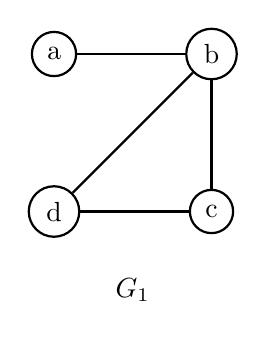
\begin{tikzpicture}
	\begin{scope}[every node/.style={circle,thick,draw}]
	\node (a) at (0,2) {a};
	\node (b) at (2,2) {b};
	\node (c) at (2,0) {c};
	\node (d) at (0,0) {d};
	\end{scope}
	\begin{scope}[every edge/.style={draw=black,thick}]
	\path (a) edge (b);
	\path (b) edge (c);
	\path (b) edge (d);
	\path (c) edge (d);
	\end{scope}
	\node () at (1,-1) {$G_1$};
	\end{tikzpicture}
	\hspace{1.5cm}
	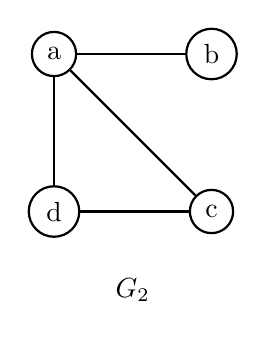
\begin{tikzpicture}
	\begin{scope}[every node/.style={circle,thick,draw}]
	\node (1) at (0,2) {a};
	\node (2) at (2,2) {b};
	\node (3) at (2,0) {c};
	\node (4) at (0,0) {d};
	\end{scope}
	\begin{scope}[every edge/.style={draw=black,thick}]
	\path (1) edge (2);
	\path (1) edge (3);
	\path (1) edge (4);
	\path (3) edge (4);
	\end{scope}
	\node () at (1,-1) {$G_2$};
	\end{tikzpicture}
	\caption{Nice pictures}
	\label{tikz:graphs}
\end{figure}


\begin{figure}
	\centering
	\begin{tikzpicture}[node distance=6cm]
	\node (a) [rect] {A Big Blue Block};
	\node (b) [oval, right of=a] {And His Oval Friend};
	\draw [line] (a) -- (b);
	\end{tikzpicture}
	\caption{Nice pictures}
	\label{tikz:graphs}
\end{figure}


\chapter{Technology Review}
About seven to ten pages.
\begin{itemize}
	\item Describe each of the technologies you used at a conceptual level. Standards, Database Model (e.g. MongoDB, CouchDB), XMl, WSDL, JSON, JAXP.
	\item Use references (IEEE format, e.g. [1]), Books, Papers, URLs (timestamp) – sources should be authoritative. 
\end{itemize}

\section{XML}
Here's some nicely formatted XML:
\begin{minted}{xml}
<this>
<looks lookswhat="good">
Good
</looks>
</this>
\end{minted}

\chapter{System Design}
As many pages as needed.
\begin{itemize}
	\item Architecture, UML etc. An overview of the different components of the system. Diagrams etc… Screen shots etc.
\end{itemize}

\begin{table}[h]
	\centering
	\begin{tabular}{x{2cm}p{3cm}}
		\toprule \\
		Column 1 & Column 2 \\
		\midrule \\
		Rows 2.1 & Row 2.2 \\
		\bottomrule
	\end{tabular}
	\caption{A table.}
	\label{table:mytable}
\end{table}

\chapter{System Evaluation}
As many pages as needed.
\begin{itemize}
	\item Prove that your software is robust. How? Testing etc. 
	\item Use performance benchmarks (space and time) if algorithmic.
	\item Measure the outcomes / outputs of your system / software against the objectives from the Introduction.
	\item Highlight any limitations or opportuni-ties in your approach or technologies used.
\end{itemize}

\chapter{Conclusion}
About three pages.

\begin{itemize}
	\item Briefly summarise your context and ob-jectives (a few lines).
	\item Highlight your findings from the evalua-tion section / chapter and any opportuni-ties identified.
\end{itemize}

